\subsection{Bandwidth Reduction Protocol}
\label{sec:protocol}
The second major part of our technique is the reduction protocol between the mobile device and the proxy server. It brings together all the components described in the previous sections. Each time a new page is requested by the mobile browser, the following protocol is performed (Figure \ref{fig:protocol}):

\begin{enumerate}
\item Mobile proxy-client sends an HTTP request to the proxy server.
\item Proxy server relays this request to the proper web server.
\item Proxy server performs chunking and fingerprinting of the chunks for all the received web content. It sends all the fingerprints to the mobile device.
\item Mobile proxy-client checks its cache for the fingerprints, and creates a list of those it needs. It sends this list to the proxy server.
\item Proxy server creates a list of the needed chunks according to the received needed fingerprints. It sends this list back to the mobile device.
\item Mobile proxy-client reconstructs the entire requested page from its cache contents and the received list of needed chunks.
\end{enumerate}

\begin{figure}[h] 
\centering 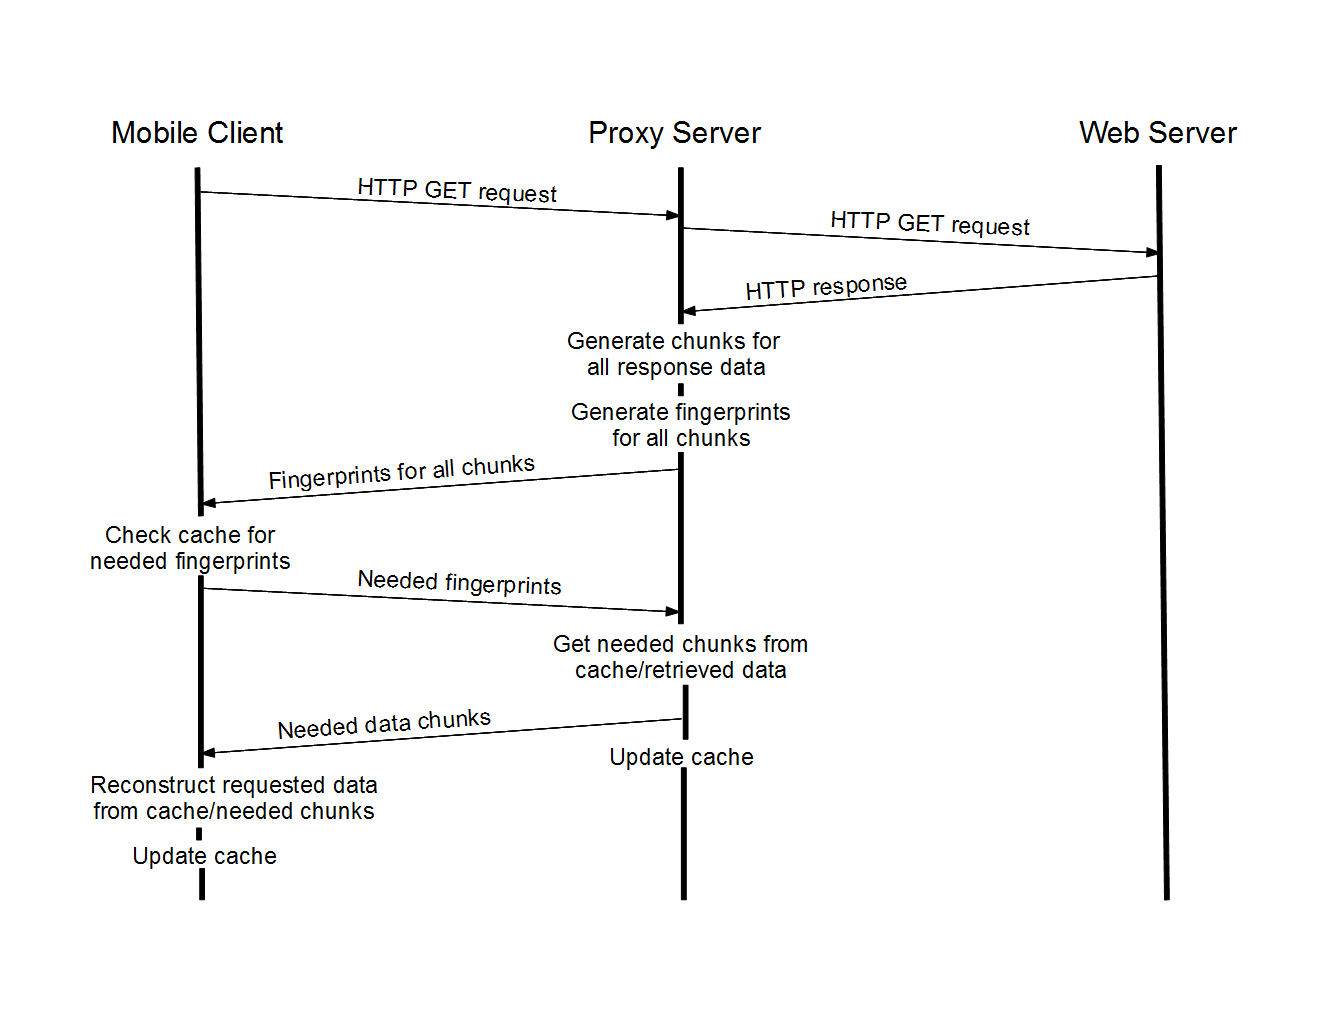
\includegraphics[scale=0.40]{images/protocol_diagram.png}
\caption{The Bandwidth Reduction Protocol as Part of the Whole System.}
\label{fig:protocol}
\end{figure}

Our protocol uses standard HTTP GET requests and does not require changes to web server configurations. It also does not alter the mobile browser front-end and simply requires the mobile proxy-client as the interface to the proxy server.







